\chapter{Brief Review of Electromagnetics}

%\setcounter{page}{1}

\renewcommand{\thefootnote}{\fnsymbol{footnote}}
\footnotetext{Lecture notes by John Schneider.  {\tt
em-review.tex}}

\section{Introduction}

The specific equations on which the finite-difference time-domain
(FDTD) method is based will be considered in some detail later.  The
goal here is to remind you of the physical significance of the
equations to which you have been exposed in previous courses on
electromagnetics.

In some sense there are just a few simple premises which underlie all
electromagnetics.  One could argue that electromagnetics is simply
based on the following:
\begin{enumerate}
\item Charge exerts force on other charge.
\item Charge in motion exerts a force on other charge in motion.
\item All material is made up of charged particles.
\end{enumerate}
Of course translating these premises into a corresponding mathematical
framework is not trivial.  However one should not lose sight of the
fact that the math is trying to describe principles that are
conceptually rather simple.

\section{Coulomb's Law and Electric Field}

Coulomb studied the electric force on charged particles.  As depicted
in Fig.\ \ref{fig:coulomb}, given two
discrete particles carrying charge $Q_1$ and $Q_2$, the force
experienced by $Q_2$ due to $Q_1$ is along the line joining $Q_1$ and
$Q_2$.
\begin{figure}
  \begin{center}
  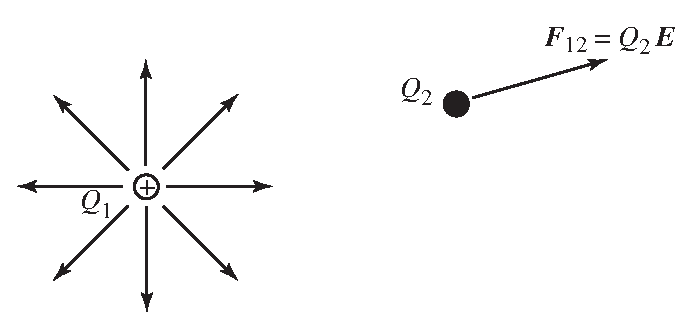
\epsfig{width=4.in,file=Figures/Em-review/coulomb.eps}
  \end{center}
  \caption{The force experienced by charge $Q_2$ due to charge $Q_1$ is
  along the line which pass through both charges.  The direction of
  the force is dictate by the signs of the charges.  Electric field is
  assumed to point radially away from positive charges as is indicated
  by the lines pointing away from $Q_1$ (which is assumed here to
  be positive).}
  \label{fig:coulomb}
\end{figure}
The force is proportional to the charges and inversely proportional to
the square of the distance between the charges.  A proportionality
constant is needed to obtain Coulomb's law which gives the equation of
the force on $Q_2$ due to $Q_1$:
\begin{equation}
  \mathbf{F}_{12} = \unitvec{12}
                    \frac{1}{4\pi\epsilon_0}
                    \frac{Q_1 Q_2}{R_{12}^2}
  \label{eq:coulomb}
\end{equation}
where $\unitvec{12}$ is a unit vector pointing from $Q_1$ to $Q_2$,
$R_{12}$ is the distance between the charges, and $1/4\pi\epsilon_0$
is the proportionality constant.  The constant $\epsilon_0$ is known
as the permittivity of free space and equals approximately
$8.854\times 10^{-12}$ F/m.  Charge is expressed in units of Coulombs
(C) and can be either negative or positive.  When the two charges have
like signs, the force will be repulsive: $\mathbf{F}_{12}$ will
be parallel to $\unitvec{12}$.  When the charges are of opposite sign,
the force will be attractive so that $\mathbf{F}_{12}$ will be
anti-parallel to $\unitvec{12}$.

There is a shortcoming with \refeq{eq:coulomb} in that it implies
action at a distance.  It appears from this equation that the force
$\mathbf{F}_{12}$ is established instantly.  From this equation one
could assume that a change in the distance $R_{12}$ results in an
instantaneous change in the force $\mathbf{F}_{12}$, but this is not
the case.  A finite amount of time is required to communicate the
change in location of one charge to the other charge (similarly, it
takes a finite amount of time to communicate a change in the quantity
of one charge to the other charge).  To overcome this shortcoming it
is convenient to employ the concept of fields.  Instead of $Q_1$
producing a force directly on $Q_2$, $Q_1$ is said to produce a field.
This field then produces a force on $Q_2$.  The field produced by
$Q_1$ is independent of $Q_2$---it exists whether or not $Q_2$ is
there to experience it.

In the static case, the field approach does not appear to have any
advantage over the direct use of Coulomb's law.  This is because for
static charges Coulomb's law is correct.  Fields must be time-varying
for the distinction to arise.  Nevertheless, to be consistent with the
time-varying case, fields are used in the static case as well.  The
electric field produced by the point charge $Q_1$ is
\begin{equation}
  \Evec_1 = \unitvec{r} \frac{Q_1}{4 \pi\epsilon_0 r^2}
  \label{eq:eField}
\end{equation}
where $\unitvec{r}$ is a unit vector which points radially away from
the charge and $r$ is the distance from the charge.  The electric
field has units of volts per meter (V/m).

To find the force on $Q_2$, one merely takes the charge times the
electric field: $\mathbf{F}_{12}=Q_2 \Evec_1$.  In general, the force
on any charge $Q$ is the product of the charge and the electric field
at which the charge is present, i.e., $\mathbf{F}=Q \Evec$.

\section{Electric Flux Density}

All material is made up of charged particles.  The material may be
neutral overall because it has as many positive charges as negative
charges.  Nevertheless, there are various ways in which the positive
and negative charges may shift slightly within the material, perhaps
under the influence of an electric field.  The resulting
charge separation will have an effect on the overall electric field.
Because of this it is often convenient to introduce a new field known
as the electric flux density, $\Dvec$, which has units of Coulombs per
square meter (C/m$^2$).\footnote{Note that not everybody advocates
using the $\Dvec$ field.  See for example Volume II of {\em The
Feynman Lectures on Physics}, R. P. Feynman, R. B. Leighton, and
M. Sands, Addison-Wesley, 1964.  Feynman only uses $\Evec$ and never
resorts to $\Dvec$.}  Essentially the $\Dvec$ field ignores the local
effects of charge which is bound in a material.

In free space, the electric field and the electric flux density are
related by
\begin{equation}
  \Dvec = \epsilon_0\Evec.
\end{equation}
Gauss's law states that
integrating $\Dvec$ over a closed surface yields the enclosed free
charge
\begin{equation}
  \oint_S \Dvec\cdot \mathbf{ds} = Q_{\mbox{\scriptsize enc}}
  \label{eq:gauss}
\end{equation}
where $S$ is the closed surface, $\mathbf{ds}$ is an incremental
surface element whose normal is directed radially outward, and
$Q_{\mbox{\scriptsize enc}}$ is the enclosed charge.  As an example,
consider the electric field given in \refeq{eq:eField}.  Taking $S$ to
be a spherical surface with the charge at the center, it is simple to
perform the integral in \refeq{eq:gauss}:
\begin{equation}
  \oint_S \Dvec\cdot \mathbf{ds} =
  \int_{\theta=0}^\pi\int_{\phi=0}^{2\pi}
    \epsilon_0 \frac{Q_1}{4 \pi\epsilon_0 r^2}\unitvec{r} \cdot
    \unitvec{r} r^2\sin\theta \, d\phi \, d\theta = Q_1.
  \label{eq:gaussExamp}
\end{equation}
The result is actually independent of the surface chosen (provided it
encloses the charge), but the integral is especially easy to perform
for a spherical surface.

We want the integral in \refeq{eq:gauss} always to equal the enclosed
charge as it does in free space.  However, things are more complicated
when material is present.  Consider, as shown in Fig.\
\ref{fig:platesFree}, two large parallel plates which carry uniformly
distributed charge of equal magnitude but opposite sign.  
\begin{figure}
  \begin{center}
  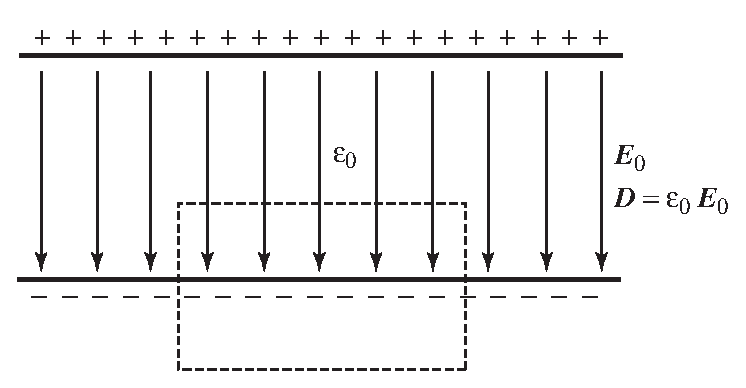
\epsfig{width=4.5in,file=Figures/Em-review/parallel-plates.eps}
  \end{center}
  \caption{Charged parallel plates in free space.  The dashed line
  represents the integration surface $S$.}
  \label{fig:platesFree}
\end{figure}
The dashed line represents an integration surface $S$ which is assumed
to be sufficiently far from the edges of the plate so that the field
is uniform over the top of $S$.  This field is identified as
$\Evec_0$.  The fields are zero outside of the plates and are
tangential to the sides of $S$ within the plates.  Therefore the only
contribution to the integral would be from the top of $S$.  The result
of the integral $\oint_S \epsilon_0\Evec\cdot \mathbf{ds}$ 
is the negative charge enclosed by the surface (i.e., the negative
charge on the bottom plate which falls within $S$).

Now consider the same plates, carrying the same charge, but with a
material present between the plates.  Assume this material is
``polarizable'' such that the positive and negative charges can shift
slightly.  The charges are not completely free to move---they are
bound charges.  The positive charges will be repelled by the top plate
and attracted to the bottom plate.  Conversely, the negative charges
will be repelled by the bottom plate and attracted to the top plate.
This scenario is depicted in Fig.\ \ref{fig:platesMat}.
\begin{figure}
  \begin{center}
  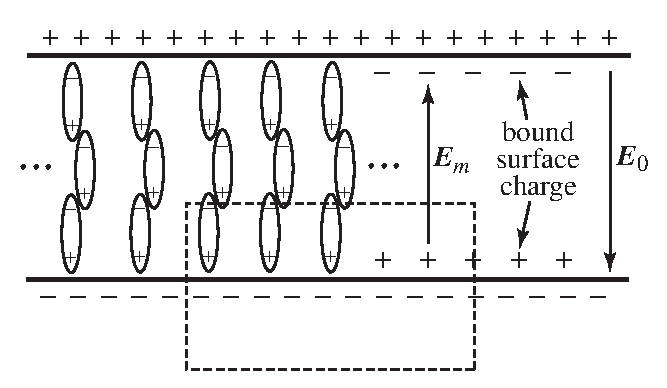
\epsfig{width=4.5in,file=Figures/Em-review/parallel-plates-dielectric.eps}
  \end{center} \caption{Charged parallel plates with a polarizable
  material present between the plates.  The elongated objects
  represent molecules whose charge orientation serves to produce a net
  bound negative charge layer at the top plate and a bound positive
  charge layer at the bottom plate.  In the interior, the positive and
  negative bound charges cancel each other.  It is only at the surface
  of the material where one must account for the bound charge.  Thus,
  the molecules are not drawn throughout the figure.  Instead, as
  shown toward the right side of the figure, merely the bound charge
  layer is shown.  The free charge on the plates creates the electric
  field $\Evec_0$.  The bound charge creates the electric field
  $\Evec_m$ which opposes $\Evec_0$ and hence diminishes the total
  electric field. The dashed line again represents the integration
  surface $S$.}  \label{fig:platesMat}
\end{figure}

With the material present the electric field due to the charge on the
plates is still $\Evec_0$, i.e., the same field as existed in Fig.\
\refeq{fig:platesFree}.  However, there is another field present due
to the displacement of the bound charge in the polarizable material
between the plates.  The polarized material effectively acts to
establish a layer of positive charge adjacent to the bottom plate and
a layer of negative charge adjacent to the top plate.  The field due
to these layers of charge is also uniform but it is in the opposite
direction of the field caused by the ``free charge'' on the plates.
The field due to bound charge is labeled $\Evec_m$ in Fig.\
\refeq{fig:platesMat}.  The total field is the sum of the fields due
to the bound and free charges, i.e., $\Evec = \Evec_0 + \Evec_m$.
Because $\Evec_0$ and $\Evec_m$ are anti-parallel, the magnitude of
the total electric field $\Evec$ will be less than $\Evec_0$.

Since the material is neutral, we would like the integral of the
electric flux over the surface $S$ to yield just the enclosed charge
on the bottom plate---not the bound charge due to the material.  In
some sense this implies that the integration surface cannot separate
the positive and negative bound charge of any single molecule.  Each
molecule is either entirely inside or outside the integration surface.
Since each molecule is neutral, the only contribution to the integral
will be from the free charge on the plate.

With the material present, the integral of $\oint_S
\epsilon_0\Evec\cdot \mathbf{ds}$ yields too little charge.  This is
because, as stated above, the total electric field $\Evec$ is less
than it would be if only free space were present.  To correct for the
reduced field and to obtain the desired result, the electric flux
density is redefined so that it accounts for the presence of the
material.  The more general expression for the electric flux density
is
\begin{equation}
 \Dvec = \epsilon_r\epsilon_0\Evec = \epsilon\Evec
 \label{eq:eAndD}
\end{equation}
where $\epsilon_r$ is the relative permittivity and $\epsilon$ is
called simply the permittivity.  By accounting for the permittivity of
a material, Gauss's law is always satisfied.

In \refeq{eq:eAndD}, $\Dvec$ and $\Evec$ are related by a scalar
constant.  This implies that the $\Dvec$ and $\Evec$ fields are
related by a simple proportionality constant for all frequencies, all
orientations, and all field strengths.  Unfortunately the real world
is not so simple.  Clearly if the electric field is strong enough, it
would be possible to tear apart the bound positive and negative
charges.  Since charges have some mass, they do not react the same way
at all frequencies.  Additionally, many materials may have some
structure, such as crystals, where the response in one direction is
not the same in other directions.  Nevertheless, Gauss's law is the
law and thus always holds.  When things get more complicated one must
abandon a simple scalar for the permittivity and use an appropriate
form to ensure Gauss's law is satisfied.  So, for example, it may be
necessary to use a tensor for permittivity that is directionally
dependent.  However, with the exception of frequency-dependent
behavior (i.e., dispersive materials), we will not be pursuing those
complications.  A scalar permittivity will suffice.

\section{Static Electric Fields}

Ignoring possible nonlinear behavior of material, superposition holds
for electromagnetic fields.  Therefore we can think of any
distribution of charges as a collection of point charges.  We can get
the total field by summing the contributions from all the charges (and
this summing will have to be in the form of an integration if the
charge is continuously distributed).

Note from \refeq{eq:eField} that the field associated with a point
charge merely points radially away from the charge.  There is no
``swirling'' of the field.  If we have more than a single charge, the
total field may bend, but it will not swirl.  Imagine a tiny wheel
with positive charge distributed around its circumference.  The wheel
hub of the wheel is held at a fixed location but the wheel is free to
spin about its hub.  For static electric fields, no matter where we
put this wheel, there would be no net force on the wheel to cause it
to spin.  There may be a net force pushing the entire wheel in a
particular direction (a translational force), but the forces which are
pushing the wheel to spin in the clockwise direction are balanced by
the forces pushing the wheel to spin in the counterclockwise
direction.

Another property of electrostatic fields is that the electric flux
density only begins or terminates on free charge.  If there is no
charge present, the lines of flux continue.

The lack of swirl in the electric field and the source of electric
flux density are fairly simple concepts.  However, to be able to
analyze the fields properly, one needs a mathematical statement of
these concepts.  The appropriate statements are
\begin{equation}
  \nabla\times\Evec=0
  \label{eq:curlE}
\end{equation}
and
\begin{equation}
  \nabla\cdot\Dvec=\rho_v
  \label{eq:divD}
\end{equation}
where $\nabla$ is the del or nabla operator and $\rho_v$ is the
electric charge density (with units of C/m$^3$).  Equation
\refeq{eq:curlE} is the curl of the electric field and \refeq{eq:divD}
is the divergence of the electric flux density.  These two equations
are discussed further in the following section.

\section{Gradient, Divergence, and Curl}

The del operator is independent of the coordinate system
used---naturally the behavior of the fields should not depend on the
coordinate system used to describe the field.  Nevertheless, the del
operator can be expressed in different coordinates systems.  In
Cartesian coordinates del is
\begin{equation}
  \nabla \equiv \unitvec{x} \frac{\partial}{\partial x} +
                \unitvec{y} \frac{\partial}{\partial y} +
                \unitvec{z} \frac{\partial}{\partial z}
\end{equation}
where the symbol $\equiv$ means ``defined as.''

Del acting on a scalar field produces the gradient of the field.
Assuming $f$ is a some scalar field, $\nabla f$ produces the vector
field given by 
\begin{equation}
  \nabla f = \unitvec{x} \frac{\partial f}{\partial x} +
             \unitvec{y} \frac{\partial f}{\partial y} +
             \unitvec{z} \frac{\partial f}{\partial z}.
\end{equation}
The gradient of $f$ points in the direction of greatest change and is
proportional to the rate of change.  Assume we wish to find the amount
of change in $f$ for a small movement $dx$ in the $x$ direction.  This
can be obtained via $\nabla f \cdot \unitvec{x} dx$, to wit
\begin{equation}
  \nabla f \cdot \unitvec{x} dx = \frac{\partial f}{\partial x} dx
    = \mbox{(rate of change in $x$ direction)}\times
      \mbox{(movement in $x$ direction)}.
\end{equation}
This can be generalized for movement in an arbitrary direction.
Letting an incremental small length be given by
\begin{equation}
  \mathbf{d\ell} = \unitvec{x} dx + \unitvec{y} dy + \unitvec{z} dz,
\end{equation}
the change in the field realized by moving an amount $\mathbf{d\ell}$
is
\begin{equation}
  \nabla f\cdot\mathbf{d\ell} = 
     \frac{\partial f}{\partial x} dx +
     \frac{\partial f}{\partial y} dy +
     \frac{\partial f}{\partial z} dz.
\end{equation}

Returning to \refeq{eq:divD}, when the del operator is dotted with a
vector field, one obtains the divergence of that field.  Divergence
can be thought of as a measure of ``source'' or ``sink'' strength of the
field at a given point.  The divergence of a vector field is a scalar
field given by
\begin{equation}
 \nabla \cdot \Dvec = \frac{\partial D_x}{\partial x} +
     \frac{\partial D_y}{\partial y} +
     \frac{\partial D_z}{\partial z}.
\end{equation}
Let us consider a finite-difference approximation of this divergence
in the $xy$-plane as shown in Fig.\ \ref{fig:div}.
\begin{figure}
  \begin{center}
  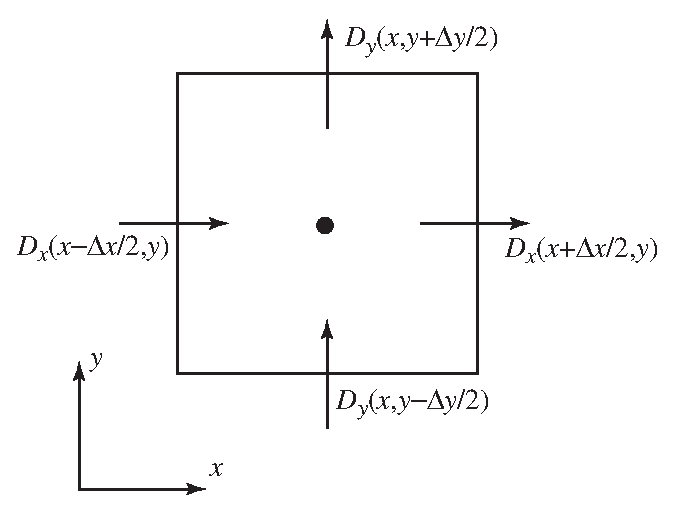
\epsfig{width=3.5in,file=Figures/Em-review/discrete-divergence.eps}
  \end{center}
  \caption{Discrete approximation to the divergence taken in the
  $xy$-plane. \label{fig:div}}  
\end{figure}
Here the divergence is measured over a small box where the field is
assumed to be constant over each edge of the box.  The derivatives can
be approximated by central differences:
\begin{equation}
  \frac{\partial D_x}{\partial x} +
  \frac{\partial D_y}{\partial y} \approx 
  \frac{D_x\left(x+\frac{\Delx}{2},y\right)
       -D_x\left(x-\frac{\Delx}{2},y\right)}{\Delx} +
  \frac{D_y\left(x,y+\frac{\Dely}{2}\right)
       -D_y\left(x,y-\frac{\Dely}{2}\right)}{\Dely}
  \label{eq:divII}
\end{equation}
where this is exact as $\Delx$ and $\Dely$ go to zero.
Letting $\Delx=\Dely=\delta$, \refeq{eq:divII} can be written
\begin{equation}
  \frac{\partial D_x}{\partial x} +
  \frac{\partial D_y}{\partial y} \approx 
  \frac{1}{\delta}
  \left(D_x\left(x+\frac{\delta}{2},y\right) -
        D_x\left(x-\frac{\delta}{2},y\right) +
        D_y\left(x,y+\frac{\delta}{2}\right) -
        D_y\left(x,y-\frac{\delta}{2}\right)\right).
  \label{eq:divIII}
\end{equation}
Inspection of \refeq{eq:divIII} reveals that the divergence is
essentially a sum of the field over the faces with the appropriate
sign changes.  Positive signs are used if the field is assumed to
point out of the box and negative signs are used when the field is
assumed to point into the box.  If the sum of these values is
positive, that implies there is more flux out of the box than into it.
Conversely, if the sum is negative, that means more flux is flowing
into the box than out.  If the sum is zero, there must be as much flux
flowing into the box as out of it (that does not imply necessarily that,
for instance, $D_x\left(x+\delta/2,y\right)$ is equal to
$D_x\left(x-\delta/2,y\right)$, but rather that the sum of all four
fluxes must be zero).

Equation \refeq{eq:divD} tells us that the electric flux density has
zero divergence except where there is charge present (as specified by
the charge-density term $\rho_v$).  If the charge density is zero, the
total flux entering some small enclosure must also leave it.  If the
charge density is positive at some point, more flux will leave a small
enclosure surrounding that point than will enter it.  On the other
hand, if the charge density is negative, more flux will enter the
enclosure surrounding that point than will leave it.

Finally, let us consider \refeq{eq:curlE} which is the curl of the
electric field.  In Cartesian coordinates it is possible to treat this
operation as simply the cross product between the vector operator
$\nabla$ and the vector field $\Evec$:
\begin{equation}
  \nabla\times\Evec =
  \left|
  \begin{array}{ccc}
     \unitvec{x} & \unitvec{y} & \unitvec{z} \\
     \frac{\partial}{\partial x} &
     \frac{\partial}{\partial y} &
     \frac{\partial}{\partial z} \\
     E_x & E_y & E_z
  \end{array}
  \right|
  =
  \unitvec{x}\left(\frac{\partial E_z}{\partial y} -
                   \frac{\partial E_y}{\partial z}\right) +
  \unitvec{y}\left(\frac{\partial E_x}{\partial z} -
                   \frac{\partial E_z}{\partial x}\right) +
  \unitvec{z}\left(\frac{\partial E_y}{\partial x} -
                   \frac{\partial E_x}{\partial y}\right).
  \label{eq:curl}
\end{equation}
Let us consider the behavior of only the $z$ component of this
operator which is dictated by the field in the $xy$-plane as shown in
Fig.\ \ref{fig:curl}.
\begin{figure}
  \begin{center}
  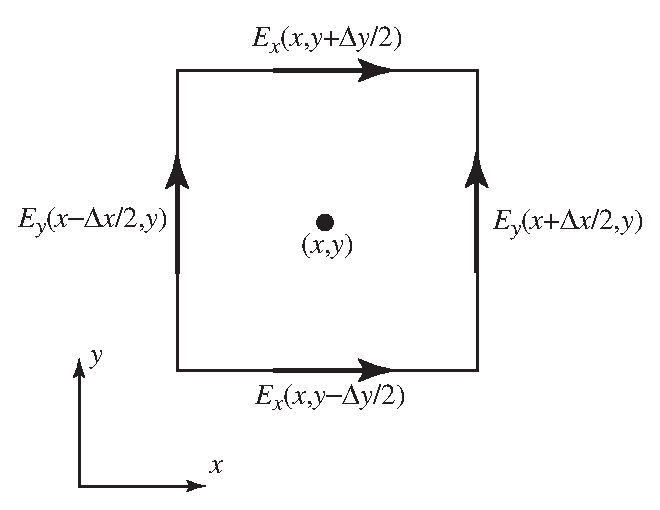
\epsfig{width=3.5in,file=Figures/Em-review/discrete-curl.eps}
  \end{center}
  \caption{Discrete approximation to the curl taken in the
  $xy$-plane. \label{fig:curl}}
\end{figure}
The $z$-component of $\nabla\times\Evec$ can be written as
\begin{equation}
  \frac{\partial E_y}{\partial x} -
  \frac{\partial E_x}{\partial y} \approx 
  \frac{E_y\left(x+\frac{\Delx}{2},y\right)
       -E_y\left(x-\frac{\Delx}{2},y\right)}{\Delx} -
  \frac{E_x\left(x,y+\frac{\Dely}{2}\right)
       -E_x\left(x,y-\frac{\Dely}{2}\right)}{\Dely}.
  \label{eq:curlII}
\end{equation}
The finite-difference approximations of the derivatives are again
based on the fields on the edges of a box surrounding the point of
interest.  However, in this case the relevant fields are tangential to
the edges rather than normal to them.  Again letting
$\Delx=\Dely=\delta$, \refeq{eq:curlII} can be written
\begin{equation}
  \frac{\partial E_y}{\partial x} -
  \frac{\partial E_x}{\partial y} \approx 
  \frac{1}{\delta}
  \left(E_y\left(x+\frac{\delta}{2},y\right) -
        E_y\left(x-\frac{\delta}{2},y\right) -
        E_x\left(x,y+\frac{\delta}{2}\right) +
        E_x\left(x,y-\frac{\delta}{2}\right)\right).
  \label{eq:curlIII}
\end{equation}
In the sum on the right side the sign is positive if the vector
component points in the counterclockwise direction (relative to
rotations about the center of the box) and is negative if the vector
points in the clockwise direction.  Thus, if the sum of these vector
components is positive, that implies that the net effect of these
electric field vectors is to tend to push a positive charge in the
counterclockwise direction.  If the sum were negative, the vectors
would tend to push a positive charge in the clockwise direction.  If
the sum is zero, there is no tendency to push a positive charge around
the center of the square (which is not to say there would not be a
translation force on the charge---indeed, if the electric field is
non-zero, there has to be some force on the charge).

\section{Laplacian}

In addition to the gradient, divergence, and curl, there is one more
vector operator to consider.  There is a vector identity that the curl
of the gradient of any function is identically zero
\begin{equation}
  \nabla\times\nabla f = 0.
  \label{eq:vecIdent}
\end{equation}
This is simple to prove by merely performing the operations in
Cartesian coordinates.  One obtains several second-order partial
derivatives which cancel if the order of differentiation is switched.
Recall that for a static distribution of charges, $\nabla\times\Evec=0$.
Since the curl of the electric field is zero, it should be possible to
represent the electric field as the gradient of some scalar function
\begin{equation}
  \Evec = -\nabla V.
  \label{eq:potential}
\end{equation}
The scalar function $V$ is the electric potential and the negative
sign is used to make the electric field point from higher potential to
lower potential (by historic convention the electric field points away
from positive charge and toward negative charge).  By expressing the
electric field this way, the curl of the electric field is guaranteed
to be zero.

Another way to express the relationship between the electric field and
the potential is via integration.  Consider movement from an arbitrary
point $a$ to an arbitrary point $b$.  The change in potential between
these two points can be expressed as
\begin{equation}
  V_b-V_a = \int_a^b \nabla V \cdot \mathbf{d\ell}.
  \label{eq:potentialInt}
\end{equation}
The integrand represent the change in the potential for a movement
$\mathbf{d\ell}$ and the integral merely sums the changes over the
path from $a$ to $b$.  However, the change in potential must also be
commensurate with the movement in the direction of, or against, the
electric field.  If we move against the electric field, potential
should go up.  If we move along the electric field, the potential
should go down.  In other words, the incremental change in potential
for a movement $\mathbf{d\ell}$ should be
$dV=-\Evec\cdot\mathbf{d\ell}$ (if the movement $\mathbf{d\ell}$ is
orthogonal to the electric field, there should be no change in the
potential).  Summing change in potential over the entire path yields
\begin{equation}
  V_b-V_a = - \int_a^b \Evec \cdot \mathbf{d\ell}.
  \label{eq:potentialIntII}
\end{equation}
The integrals in \refeq{eq:potentialInt} and \refeq{eq:potentialIntII}
can be equated.  Since the equality holds for any two arbitrary points,
the integrands must be equal and we are again left with $\Evec =
-\nabla V$. 

The electric flux density can be related to the electric field via
$\Dvec=\epsilon\Evec$ and the behavior of the flux density $\Dvec$ is
dictated by $\nabla\cdot\Dvec=\rho_v$.  Combining these with
\refeq{eq:potential} yields
\begin{equation}
  \Evec = \frac{1}{\epsilon}\Dvec = -\nabla V.
\end{equation}
Taking the divergence of both sides yields
\begin{equation}
  \frac{1}{\epsilon}\nabla\cdot\Dvec =  
  \frac{1}{\epsilon} \rho_v =
  -\nabla\cdot\nabla V.
\end{equation}
Rearranging this yields Poisson's equation given by
\begin{equation}
  \nabla^2 V = -\frac{\rho_v}{\epsilon}
  \label{eq:poisson}
\end{equation}
where $\nabla^2$ is the Laplacian operator
\begin{equation}
  \nabla^2 \equiv \nabla\cdot\nabla =
     \frac{\partial^2}{\partial x^2} +
     \frac{\partial^2}{\partial y^2} +
     \frac{\partial^2}{\partial z^2}.
\end{equation}
Note that the Laplacian is a scalar operator.  It can act on a scalar
field (such as the potential $V$ as shown above) or it can act on a
vector field as we will see later.  When it acts on a vector field,
the Laplacian acts on each component of the field.

In the case of zero charge density, \refeq{eq:poisson} reduces to
Laplace's equation
\begin{equation}
  \nabla^2 V = 0.
\end{equation}  
We have a physical intuition about what gradient, divergence, and curl
are telling us, but what about the Laplacian?  To answer this,
consider a function of a single variable.

Given the function $V(x)$, we can ask if the function at some point is
greater than, equal to, or less than the average of its neighboring
values.  The answer can be expressed in terms of the value of the
function at the point of interest and the average of samples to either
side of that central point:
\begin{equation}
  \frac{V(x+\delta) + V(x-\delta)}{2} - V(x) =
  \left\{
    \begin{array}{ll}
      \mbox{positive}&\mbox{if center point less than average of neighbors} \\
      \mbox{zero} &\mbox{if center point equals average of neighbors} \\
      \mbox{negative}&\mbox{if center point greater than average of neighbors}
    \end{array}
  \right.
  \label{eq:avg}
\end{equation}
Here the left-most term represents the average of the neighboring
values and $\delta$ is some displacement from the central point.
Equation \refeq{eq:avg} can be normalized by $\delta^2/2$ without changing
the basic tenants of this equation.  Performing that normalization and
rearranging yields
\begin{eqnarray}  
  \frac{1}{\delta^2/2}
  \left\{
    \frac{V(x+\delta) + V(x-\delta)}{2} - V(x)
  \right\}
  &=&
  \frac{1}{\delta^2}
  \left\{
    (V(x+\delta) - V(x)) - (V(x)-V(x-\delta))
  \right\} \nonumber
 \\
  &=&
  \frac{
    \frac{V(x+\delta) - V(x)}{\delta} -
    \frac{V(x)-V(x-\delta)}{\delta}}{\delta}  \nonumber
 \\
  &\approx&
  \frac{
    \frac{\partial V(x+\delta/2)}{\partial x} -
    \frac{\partial V(x-\delta/2)}{\partial x}}{\delta} \nonumber
 \\
  &\approx&
  \frac{\partial^2 V(x)}{\partial x^2}.
\end{eqnarray}
Thus the second partial derivative can be thought of as a way of
measuring the field at a point relative to its neighboring points.
You should already have in mind that if the second derivative is
negative, a function is tending to curve downward.  Second derivatives
are usually discussed in the context of curvature.  However, you
should also think in terms of the field at a point and its neighbors.
At points where the second derivative is negative those points are
higher than the average of their neighboring points (at least if the
neighbors are taken to be an infinitesimally small distance away).

In lieu of these arguments, Poisson's equation \refeq{eq:poisson}
should have physical significance.  Where the charge density is zero,
the potential cannot have a local minima or maxima.  The potential is
always equal to the average of the neighboring points.  If one
neighbor is higher, the other must be lower (and this concept easily
generalizes to higher dimensions).  Conversely, if the charge density
is positive over some region, the potential should increase as one
moves deeper into that region but the rate of increase must be such
that at any point the average of the neighbors is less than the center
point.  This behavior is illustrated in Fig.\ \ref{fig:chargeSphere}
which depicts the potential along a path through the center of a
uniform sphere of charge.
\begin{figure}
  \begin{center}
  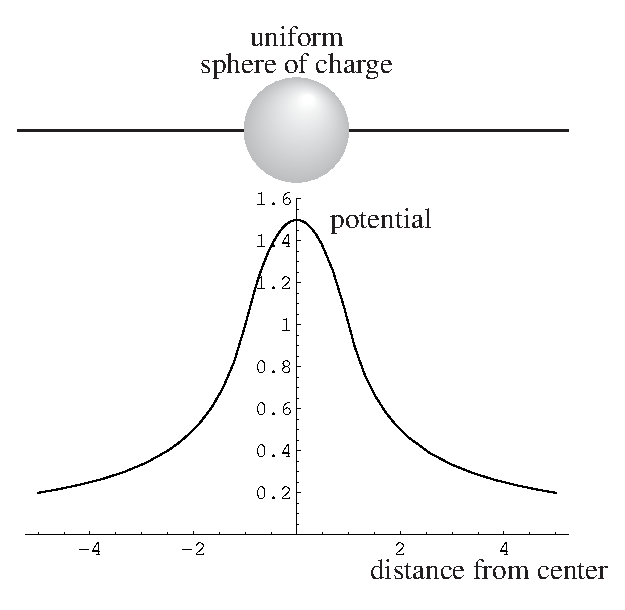
\epsfig{width=4in,file=Figures/Em-review/sphere-potential.eps}
  \end{center}
  \caption{Potential along a path which passes through a uniform
  sphere of positive charge (arbitrary units). \label{fig:chargeSphere}}
\end{figure}

\section{Gauss's and Stokes' Theorems}

Equation \refeq{eq:gauss} presented Gauss's law which stated the flux
of $\Dvec$ through a closed surface $S$ is equal to the enclosed
charge.  There is an identity in vector calculus, known as Gauss's
theorem, which states that the integral of the flux of any vector
field through a closed surface equals the integral of the divergence
of the field over the volume enclosed by the surface.  This holds for
any vector field, but using the $\Dvec$ field, Gauss's theorem states
\begin{equation}
  \oint_S \Dvec\cdot\mathbf{ds} = 
  \int_V \nabla\cdot \Dvec dv
  \label{eq:gaussTheorem}
\end{equation}
where $V$ is the enclosed volume and $dv$ is a differential volume
element.  Note that the left-hand side of \refeq{eq:gaussTheorem} is
the left-hand side of \refeq{eq:gauss}.

The right-hand side of \refeq{eq:gauss} is the enclosed charge
$Q_{\mbox{\scriptsize enc}}$ which could be determined either by
evaluating the left-hand side of \refeq{eq:gauss} or by integration of
the charge density $\rho_v$ over the volume enclosed by $S$.  (This is
similar to determining the mass of an object by integrating its mass
density over its volume.)  Thus,
\begin{equation}
  Q_{\mbox{\scriptsize enc}} =
  \int_V \rho_v dv.
  \label{eq:chargeIntegral}
\end{equation}
Equating the right-hand sides of \refeq{eq:gaussTheorem} and
\refeq{eq:chargeIntegral} yields
\begin{equation}
  \int_V \nabla\cdot \Dvec dv =
  \int_V \rho_v dv.
\end{equation}
Since this must hold over an arbitrary volume, the integrands must be
equal which yields \refeq{eq:divD}.

Another useful identity from vector calculus is Stokes' theorem which
states that the integral of a vector field over any closed path is
equal to the integral of the curl of that field over a surface which
has that path as its border.  Again, this holds for any vector field,
but using the electric field as an example one can write
\begin{equation}
  \oint_L \Evec\cdot\mathbf{d\ell} = 
  \int_S \nabla\times\Evec \cdot \mathbf{ds}.
  \label{eq:stokes}
\end{equation}
The surface normal is assumed to follow the right-hand convention so
that when the fingers of the right hand are oriented along the path of
the loop, the thumb points in the positive direction of the surface
normal.

Static electric fields are conservative which means that the net work
required to move a charge in a closed path is always zero.  Along some
portion of the path positive work would have to be done to push the
charge against the field, but this amount of work would be given back
by the field as the charge travels along the remaining portions of the
path.  The integrand on the left-hand side in \refeq{eq:stokes} is the
field dotted with an incremental length.  If the integrand were
multiplied by a unit positive charge, the integrand would represent
work, since charge times field is force and force times distance is
work.  Because the electric field is conservative, the integral on the
left-hand side of \refeq{eq:stokes} must be zero.  Naturally this
implies that the integral on the right-hand side must also be zero.
Since this holds for any loop $L$ (or, similarly, any surface $S$), the
integrand itself must be zero.  Equating the integrand to zero yields
\refeq{eq:curlE}.

\section{Electric Field Boundary Conditions}

Consider an interface between two homogeneous regions.  Because
electric flux density only begins or ends on charge, the normal
component of $\Dvec$ can only change at the interface if there is
charge on the interface, i.e., surface charge is present.  This can be
stated mathematically as
\begin{equation}
 \hat{\mathbf{n}} \cdot(\Dvec_1 - \Dvec_2) = \rho_s
\end{equation}
where $\rho_s$ is a surface charge density (C/m$^2$),
$\hat{\mathbf{n}}$ is a unit vector normal to the surface, and
$\Dvec_1$ and $\Dvec_2$ are the field to either side of the interface.
One should properly argue this boundary condition by an application of
Gauss's law for a small volume surrounding the surface, but such
details are left to other classes (this is just a review!).  If no
charge is present, the normal components must be equal
\begin{equation}
 \hat{\mathbf{n}} \cdot \Dvec_1 = \hat{\mathbf{n}} \cdot \Dvec_2.
\end{equation}

The boundary conditions on the tangential component of the electric
field can be determined by integrating the electric field over a
closed loop which is essentially a rectangle which encloses a portion
of the interface.  By letting the sides shrink to zero and keeping the
``top'' and ``bottom'' of the rectangle small but finite (so that they
are tangential to the surface), one essentially has that the field
over the top must be the same as the field over the bottom (owing to
the fact that total integral must be zero since the field is
conservative).  Stated mathematical, the boundary condition is
\begin{equation}
 \hat{\mathbf{n}} \times (\Evec_1 - \Evec_2) = 0.
\end{equation}

\section{Conductivity and Perfect Electric Conductors}

It is possible for the charge in materials to move under the influence
of an electric field such that currents flow.  If the material has a
non-zero conductivity $\sigma$, the current density is given by
\begin{equation}
  \Jvec = \sigma \Evec.
\end{equation}
The current density has units of A/m$^2$ and the conductivity has
units of S/m.

If charge is building up or decaying in a particular region, the
divergence of the current density must be non-zero.  If the divergence
is zero, that implies as much current leaves a point as enters it and
there is no build-up or decay of charge.  This can be stated as
\begin{equation}
  \nabla \cdot \Jvec = -\frac{\partial \rho_v}{\partial t}.
  \label{eq:chargeConservation}
\end{equation}
If the divergence is positive, the charge density must be decreasing
with time (so the negative sign will bring the two into agreement).
This equation is a statement of charge conservation.

Perfect electric conductors (PECs) are materials where it is assumed
that the conductivity approaches infinity.  If the fields were
non-zero in a PEC, that would imply the current was infinite.  Since
infinite currents are not allowed, the fields inside a PEC are
required to be zero.  This subsequently requires that the tangential
electric field at the surface of a PEC is zero (since tangential
fields are continuous across an interface and the fields inside the
PEC are zero).  Correspondingly, the normal component of the electric
flux density $\Dvec$ at the surface of a PEC must equal the charge
density at the surface of the PEC.  Since the fields inside a PEC are
zero, all points of the PEC must be at the same potential.

\section{Magnetic Fields}

Magnetic fields circulate around, but they do not terminate on
anything---there is no (known) magnetic charge.  Nevertheless, it is
often convenient to define magnetic charge and magnetic current.
These fictions allow one to simplify various problems such as integral
formulations of scattering problems.  However for now we will stick to
reality and say they do not exist.

The magnetic flux density $\Bvec$ is somewhat akin to the electric
field in that the force on a charge in motion is related to $\Bvec$.
If a charge $Q$ is moving with velocity $\mathbf{u}$ in a field
$\Bvec$, it experiences a force
\begin{equation}
  \mathbf{F} = Q \mathbf{u}\times\Bvec.
\end{equation}
Because $\Bvec$ determines the force on a charge, it must account for
all sources of magnetic field.  When material is present, the charge
in the material can have motion (or rotation) which influences the
magnetic flux density.

Alternatively, similar to the electric flux density, we define the
magnetic field $\Hvec$ which ignores the local effects of material.
These fields are related by
\begin{equation}
  \Bvec = \mu_r\mu_0 \Hvec = \mu\Hvec
\end{equation}
where $\mu_r$ is the relatively permeability, $\mu_0$ is the
permeability of free space equal to $4\pi\times 10^{-7}$ H/m, and
$\mu$ is simply the permeability.  Typically the relative permeability
is greater than unity (although usually only by a small amount) which
implies that when a material is present the magnetic flux density is
larger than when there is only free space.

Charge in motion is the source of magnetic fields.  If a current $I$
flows over an incremental distance $\mathbf{d\ell}$, it will produce a
magnetic field given by:
\begin{equation}
  \Hvec = \frac{I\mathbf{d\ell}\times \mathbf{a}_r}
               {4 \pi r^2}
  \label{eq:biot}
\end{equation}
where $\mathbf{a}_r$ points from the location of the filament of
current to the observation point and $r$ is the distance between the
filament and the observation point.  Equation \refeq{eq:biot} is known
as the Biot-Savart equation.  Of course, because of the conservation
of charge, a current cannot flow over just a filament and then
disappear.  It must flow along some path.  Thus, the magnetic field
due to a loop of current would be given by
\begin{equation}
  \Hvec = \oint_L\frac{I\mathbf{d\ell}\times \mathbf{a}_r}
               {4 \pi r^2}.
  \label{eq:biotIntegral}
\end{equation}
If the current was flowing throughout a volume or over a surface, the
integral would be correspondingly changed to account for the
current wherever it flowed.

From \refeq{eq:biotIntegral} one sees that currents (which are just
another way of saying charge in motion) are the source of magnetic
fields.  Because of the cross-product in \refeq{eq:biot} and
\refeq{eq:biotIntegral}, the magnetic field essentially swirls around
the current.  If one integrates the magnetic field over a closed path,
the result is the current enclosed by that path
\begin{equation}
  \oint_L \Hvec \cdot \mathbf{d\ell} = I_{\mbox{\scriptsize enc}}.
  \label{eq:hIntegral}
\end{equation}
The enclosed current $I_{\mbox{\scriptsize enc}}$ is the current that
passes through the surface $S$ which is bound by the loop $L$.

The left-hand side of \refeq{eq:hIntegral} can be converted to a
surface integral by employing Stokes' theorem while the right-hand
side can be related to the current density by integrating over the
surface of the loop.  Thus,
\begin{equation}
  \oint_L \Hvec\cdot \mathbf{d\ell} = 
  \int_S \nabla\times\Hvec \cdot \mathbf{ds} =
  I_{\mbox{\scriptsize enc}} =
  \int_S \Jvec \cdot \mathbf{ds}.
  \label{eq:hIntegralII}
\end{equation}
Since this must be true for every loop (and surface), the integrands
of the second and fourth terms can be equated.  This yields
\begin{equation}
  \nabla\times\Hvec = \Jvec.
\end{equation}

The last equation needed to characterize static fields is
\begin{equation}
  \nabla\cdot\Bvec=0.
\end{equation}
This is the mathematical equivalent of saying there is no magnetic
charge.

\section{Magnetic Field Boundary Conditions}

Note that the equation governing $\Bvec$ is similar to the equation
which governed $\Dvec$.  In fact, since the right-hand side is always
zero, the equation for $\Bvec$ is simpler.  The arguments used to
obtain the boundary condition for the normal component of the $\Dvec$
field can be applied directly to the $\Bvec$ field.  Thus, 
\begin{equation}
 \hat{\mathbf{n}} \cdot(\Bvec_1 - \Bvec_2) = 0.
\end{equation}

For the magnetic field, an integration path is constructed along
the same lines as the one used to determine the boundary condition on
the electric field.  Note that the equations governing $\Evec$ and
$\Hvec$ are similar except that the one for $\Hvec$ has a non-zero
right-hand side.  If the current density is zero over the region of
interest, then there is really no distinction between the two and one
can say that the tangential magnetic fields must be equal across a
boundary.  However, if a surface current exists on the interface,
there may be a discontinuity in the tangential fields.  The boundary
condition is given by
\begin{equation}
 \hat{\mathbf{n}} \times (\Hvec_1 - \Hvec_2)
  = \mathbf{K}
\end{equation}
where $\mathbf{K}$ is the surface current density (with units of A/m).


\section{Summary of Static Fields}

When a system is not changing with respect to time, the governing
equations are
\begin{eqnarray}
  \nabla \cdot \Dvec &=& \rho_v, \\
  \nabla \cdot \Bvec &=& 0, \\
  \nabla \times \Evec &=& 0, \\
  \nabla \times \Hvec &=& \Jvec. \label{eq:curlHdc}
\end{eqnarray}
If a loop carries a current but is otherwise neutral, it will produce
a magnetic field and only a magnetic field.  If a charge is
stationary, it will produce an electric field and only an electric
field.  The charge will not ``feel'' the loop current and the current
loop will not feel the stationary charge (at least approximately).
The magnetic field and electric field are decoupled.  If a charge $Q$
moves with velocity $\mathbf{u}$ in the presence of both an electric
field and a magnetic field, the force on the charge is the sum of the
forces due to the electric and magnetic fields
\begin{equation}
  \mathbf{F} = Q(\Evec + \mathbf{u}\times\Bvec).
\end{equation}

\section{Time Varying Fields}

What happens when a point charge moves?  We know that charge in motion
gives rise to a magnetic field, but if the charge is moving, its
associated electric field must also be changing.  Thus, when a system
is time-varying the electric and magnetic fields must be coupled.

There is a vector identity that the divergence of the curl of any
vector field is identically zero.  Taking the divergence of both sides
of \refeq{eq:curlHdc} yields
\begin{equation}
  \nabla\cdot \nabla \times \Hvec = 
  \nabla\cdot \Jvec =
  -\frac{\partial\rho_v}{\partial t}
\end{equation}
where the conservation of charge equation was used to write the last
equality.  Since the first term must be zero, this implies that 
$\partial\rho_v/\partial t$ must also be zero.  However, that
is overly restrictive.  In general, for a time-varying system, the
charge density will change with respect to time.  Therefore something
must be wrong with \refeq{eq:curlHdc} as it pertains to time-varying
fields.  It was Maxwell who recognized that by adding the temporal
derivative of the electric flux density to the right-hand side of
\refeq{eq:curlHdc} the equation would still be valid for the
time-varying case.  The correct equation is given by
\begin{equation}
  \nabla \times \Hvec = \Jvec + \frac{\partial \Dvec}{\partial t}
  \label{eq:curlHac}
\end{equation}
The term $\partial \Dvec/\partial t$ is known as the displacement
current while $\Jvec$ is typically called the conduction current.
Equation \refeq{eq:curlHac} is known as Ampere's law.

Taking the divergence of the right-hand side of \refeq{eq:curlHac}
yields
\begin{equation}
  \nabla\cdot\Jvec + \frac{\partial \nabla\cdot\Dvec}{\partial t} = 
  -\frac{\partial \rho_v}{\partial t} + 
    \frac{\partial \nabla\cdot\Dvec}{\partial t} = 
  -\frac{\partial \rho_v}{\partial t} + 
    \frac{\partial \rho_v}{\partial t}
  =  0
\end{equation}
where use was made of \refeq{eq:divD} and the conservation of charge
equation \refeq{eq:chargeConservation}.

The electromotive force (EMF) is the change in potential over some
path.  It has been observed experimentally that when a magnetic field
is time-varying there is a non-zero EMF over a closed path which
encloses the varying field (i.e., the electric field is no longer
conservative).  

The symbol $\lambda$ is often use to represent total magnetic flux
through a given surface, i.e.,
\begin{equation}
  \lambda = \int_S \Bvec\cdot\mathbf{ds}.
\end{equation}
For time-varying fields, the EMF over a closed path $L$ can be written
\begin{eqnarray}
  V_{\mbox{\scriptsize emf}} &=& \frac{d\lambda}{dt}, \\
  -\oint_L \Evec\cdot\mathbf{d\ell} &=& 
    \frac{d}{dt}\int_S \Bvec\cdot\mathbf{ds}, \\
  -\int_S \nabla\times\Evec\cdot\mathbf{ds} &=& 
    \int_S \frac{\partial\Bvec}{\partial t}\cdot\mathbf{ds},
\end{eqnarray}
where Stokes' theorem was used to write the last equation.  Since this
equality holds over any surface, the integrands must be equal.  This
yields
\begin{equation}
  \nabla\times\Evec = -\frac{\partial\Bvec}{\partial t}
\end{equation}
which is known as Faraday's law.

\section{Summary of Time-Varying Fields}

When a system is changing with respect to time, the governing
equations are
\begin{eqnarray}
\nabla \cdot \Dvec &=& \rho_v, \label{eq:divDtime} \\
\nabla \cdot \Bvec &=& 0, \\
\nabla \times \Evec &=& -\frac{\partial\Bvec}{\partial t}, 
  \label{eq:curlBtime} \\
\nabla \times \Hvec &=& \Jvec + \frac{\partial\Dvec}{\partial t}.
  \label{eq:curlHtime}
\end{eqnarray}
Note that the divergence equations are unchanged from the static
case.  The two curl equations have picked up terms which couple the
electric and magnetic fields.  Since the additional terms both
involve temporal derivatives, they go to zero in the static case and
the equations reduce to those which governed static fields.

For time-varying fields the same boundary conditions hold as in the
static case.

%%%%%%%%%%%%%%%%%%%%%%%%%%%%%%%%%%%%%%%%%%%%%%%%%%%%%%%%%%%%%%%%%%%%%%%%%
\section{Wave Equation in a Source-Free Region}

Equations \refeq{eq:divDtime}--\refeq{eq:curlHtime} provide a set of
coupled differential equations.  In the FDTD method we will be dealing
directly with the two curl equations.  We will stick to the coupled
equations and solve them directly.  However, it is also possible to
decouple these equations.  As an example, taking the curl of both
sides of 
\refeq{eq:curlBtime} yields
\begin{equation}
  \nabla \times  \nabla \times \Evec =
 -\nabla \times \frac{\partial\Bvec}{\partial t} =
 -\mu \nabla \times \frac{\partial\Hvec}{\partial t}.
  \label{eq:gettingWaveEq}
\end{equation}
There is a vector identity that the curl of the curl of any field is
given by
\begin{equation}
  \nabla \times \nabla \times \Evec =
  \nabla(\nabla\cdot\Evec) - \nabla^2 \Evec.
\end{equation}
(This is true for any field, not just the electric field as shown
here.)  In a source-free region, there is no free charge present,
$\rho_v=0$, and hence the divergence of the electric field
is zero ($\nabla\cdot\Dvec = \epsilon\nabla\cdot\Evec = 0$).
Thus \refeq{eq:gettingWaveEq} can be written
\begin{equation}
  \nabla^2 \Evec =
  \mu \frac{\partial}{\partial t} (\nabla \times \Hvec) .
\end{equation}
Keeping in mind that we are considering a source-free region so that
$J$ would be zero, we now use \refeq{eq:curlHtime} to write
\begin{eqnarray}
  \nabla^2 \Evec &=&
  \mu \frac{\partial}{\partial t} \frac{\partial\Dvec}{\partial t}, \\
  &=&
  \mu\epsilon \frac{\partial^2\Evec}{\partial t^2}. \label{eq:waveEqE}
\end{eqnarray}

Equation \refeq{eq:waveEqE} is the wave equation for the electric
field and is often written
\begin{eqnarray}
  \nabla^2 \Evec - \frac{1}{c^2} \frac{\partial^2\Evec}{\partial t^2}
  = 0
\end{eqnarray}
where $c=1/\sqrt{\mu\epsilon}$.  Had we decoupled the equations to
solve $\Hvec$ instead of $\Evec$, we would still obtain the same
equation (except with $\Hvec$ replacing $\Evec$).



%%%%%%%%%%%%%%%%%%%%%%%%%%%%%%%%%%%%%%%%%%%%%%%%%%%%%%%%%%%%%%%%%%%%%%%%%
\section{One-Dimensional Solutions to the Wave Equation
\label{sec:waveEq}} 

%\setcounter{page}{1}

The wave equation which governs either the electric or magnetic field
in one dimension in a source-free region can be written
\begin{equation}
  \frac{\partial^2 f(x,t)}{\partial x^2} 
  - \mu\epsilon\frac{\partial^2 f(x,t)}{\partial t^2} = 0.
  \label{eq:waveEqOne}
\end{equation}
We make the claim that any function $f(\xi)$ is a solution to this
equation provided that $f$ is twice differentiable and $\xi$ is
replaced with $t\pm x/c$ where $c=1/\sqrt{\mu\epsilon}$.  Thus, we
have
\begin{equation}
  f(\xi) = f(t\pm x/c) = f(x,t).
\end{equation}
The first derivatives of this function can be obtained via the chain
rule.  Keeping in mind that
\begin{eqnarray}
  \frac{\partial\xi}{\partial t} &=& 1,\\
  \frac{\partial\xi}{\partial x} &=& \pm\frac{1}{c},
\end{eqnarray}
the first derivatives can be written
\begin{eqnarray}
  \frac{\partial f(\xi)}{\partial t} \!&=&\!
    \frac{\partial f(\xi)}{\partial \xi} \frac{\partial \xi}{\partial t}
    = \frac{\partial f(\xi)}{\partial \xi}, \\
  \frac{\partial f(\xi)}{\partial x} \!&=&\!
    \frac{\partial f(\xi)}{\partial \xi} \frac{\partial \xi}{\partial x}
    = \pm\frac{1}{c} \frac{\partial f(\xi)}{\partial \xi}.
\end{eqnarray}
Employing the chain rule in a similar fashion, the second derivatives can
be written as
\begin{eqnarray}
  \frac{\partial}{\partial t} 
    \left(\frac{\partial f(\xi)}{\partial t}\right) \!&=&\!
    \frac{\partial}{\partial t} 
    \left(\frac{\partial f(\xi)}{\partial \xi}\right) =
    \frac{\partial^2 f(\xi)}{\partial \xi^2}\frac{\partial \xi}{\partial t} =
    \frac{\partial^2 f(\xi)}{\partial \xi^2}, \label{eq:waveProof}\\
  \frac{\partial}{\partial x} 
    \left(\frac{\partial f(\xi)}{\partial x}\right) \!&=&\!
    \frac{\partial}{\partial x} 
    \left(\pm\frac{1}{c} \frac{\partial f(\xi)}{\partial \xi}\right)
    = \pm\frac{1}{c} \frac{\partial^2 f(\xi)}{\partial \xi^2}
                      \frac{\partial\xi}{\partial x} 
    = \frac{1}{c^2} \frac{\partial^2 f(\xi)}{\partial \xi^2}.
   \label{eq:waveProofI}
\end{eqnarray}
Thus, \refeq{eq:waveProof} and \refeq{eq:waveProofI} show that
\begin{eqnarray}
  \frac{\partial^2 f}{\partial t^2} &=&
     \frac{\partial^2 f}{\partial \xi^2}\\
  \frac{\partial^2 f}{\partial x^2} &=&
     \frac{1}{c^2} \frac{\partial^2 f}{\partial \xi^2}.
\end{eqnarray}
Substituting these into \refeq{eq:waveEqOne} yields
\begin{equation}
  \frac{1}{c^2} \frac{\partial^2 f}{\partial \xi^2} 
  - \frac{1}{c^2} \frac{\partial^2 f}{\partial \xi^2} = 0.
\end{equation}
The two terms on the left-hand side cancel, thus satisfying the
equation.

Consider a constant argument of $f$, say $t - x/c=0$.  Assume this
argument is obtain by simultaneously having $t=0$ and $x=0$.  Now, let
time advance by one second, i.e., $t=1$ s.  How must the position $x$
change to maintain an argument of zero?  Solving for $x$ yields $x=c
(1 \mbox{\ s})$.  In other words to move along with the field so as to
maintain the value $f(0)$ (whatever that value happens to be), at time
zero, we would be at position zero.  At time one second, we would have
to have moved to the location $x=c (1 \mbox{\ s})$.  Speed is change
in position over change in time.  Thus the speed with which we are
moving is $x/t = c (1 \mbox{\ s})/(1 \mbox{\ s}) = c$.

In these notes $c$ will typically be used to represent the speed of
light in free space.  Using the permittivity and permeability of free
space, we obtain $c=1/\sqrt{\epsilon_0\mu_0}\approx 3 \times 10^8$ m/s.
